% !TEX root = ../main.tex

\chapter{量子淬火动力学中的普适临界现象}

	本章我们将证明在量子多体系统中,基态所对应的量子临界点也能够控制远离平衡态的动力学普适行为。
	这种普适行为体现在系统的量子几何的演化上。
	通过研究二次型费米系统的量子淬火动力学,我们证明了系统的量子态体积通常随时间呈现线性增长, 并且线性增长率展现出了普适的规律:它的一阶导数随着控制参数的变化在量子临界点两侧出现跳变。
	这个跳变值和系统的的绝大部分细节信息无关,只被系统的维度所决定。
	这个结果揭示了非平衡量子多体系统存在普适的动力学性质。

	\section{研究背景}
	
		在其量子多体系统中,量子相变由量子涨落而非热运动驱动,并且会在系统的基态上表现出非解析行为。
		尽管在现实世界中,物质不可能被冷却到绝对零度,也就无法到达真正的基态,但系统的低能激发态仍然会受到量子临界点的影响。
		这种影响在相图上呈现出一个V字形的, 从量子相变点向有限温度展开的量子临界区域~\cite{Sachdev1999}。
		也就是说,量子临界性并不是一个仅存在于在理论的概念, 而是一个切实存在的现象,是它决定了量子临界材料的有限温度特性~\cite{Coleman2005}。
		迄今为止,大多数研究都集中在量子临界系统的热平衡特性上,而人们对于量子临界性的非平衡特性则了解甚少~\cite{Torre2010}。
		
		非平衡物理通常比平衡态物理更为复杂和丰富。
		在量子临界性方面,人们已经做出了大量努力来探索量子临界点附近的普适动力学行为。
		其中包括量子临界点处的普适弛豫~\cite{Sachdev1997}以及由Kibble-Zurek机制~\cite{Kibble1976,Zurek1985} 控制的扫描动力学~\cite{Zurek2005,Dziarmaga2005,Damski2005}等。
		尽管这些现象和非平衡相关,但它们只涉及位于临界点上方的低能激发态, 因此与基态本身的量子临界点有着根本联系。
		相对于这些“近平衡动力学”,量子临界性在远离基态的系统中作用仍然没有被研究清楚。
		值得一提的是,最近的研究进展表明,在长程相互作用系统的量子淬火动力学中存在本征的非平衡临界标度~\cite{Titum2020,De2023}。
		本章我们将揭示,即使在像二次型自由费米子这样简单的系统中, 基态的量子相变也会导致远离基态的动力学中出现普适的非解析行为,而这种行为可以通过量子几何来刻画。
		
		为了度量量子态之间的距离,人们引入了量子几何的概念。
		它包含了两个部分的信息,一个是由贝里曲率~\cite{Bohm2003}表征的相位距离,另一个是由量子度规表征~\cite{Provost1980,Matsuura2010,Ma2010b}的幅值距离。
		相比而言,贝里曲率在拓扑物理学背景下已经被深入研究,而量子度规直到最近才受到关注。
		在实验方面,量子度规已经在各种人工量子系统中被测量研究,包括冷原子~\cite{Yi2023}、氮空位中心~\cite{Yu2019} 和超导电路~\cite{Zheng2022}等。
		现在人们已经认识到,从平带超导和超流\cite{Peotta2015,Julku2016,Peotta2023,Tian2023,Espinosa2024} 到反常霍尔效应~\cite{Gianfrate2020,Wang2021,Gao2023}、 量子Fisher信息~\cite{Braunstein1994,Zanardi2007,Hauke2016}、电子-声子相互作用~\cite{Yu2023} 以及分数量子霍尔绝缘体\cite{Parameswaran2013,Neupert2015,BMera2021,BMera20212},包括量子度规在内的整个量子几何影响着多种多样的现象~\cite{Torma2023}。
		在量子相变的背景下,量子几何也被研究过~\cite{CAROLLO20201}。
		本章我们将揭示量子度规在解释量子系统中的非平衡现象,特别是在远离基态的临界动力学中的关键作用。

	\section{模型与研究方法}
	
		\subsection{模型介绍}
	
			我们研究了一般的具有空间平移不变性的二次型费米子模型,其哈密顿量可以表示为:
			\begin{equation}
				H=\sum_k C^\dagger_k \hat{\mathcal{H}}_k C_k, \label{eq:Ham}
			\end{equation}
			其中$\hat{\mathcal{H}}_k = \vec{h}_k \cdot \vec{\sigma}$对于每个$k$都是2$\times$2的矩阵。
			$\vec{\sigma} = [\hat{\sigma}^X, \hat{\sigma}^Y, \hat{\sigma}^Z]$代表泡利矩阵, 而$\vec{h}_k = [h_k^X, h_k^Y, h_k^Z]$是三分量的矢量。
			生成和湮灭算符$C_k$和$C^\dagger_k$既可以表记两分量的费米子$C_k = [c_{\alpha, k}, c_{\beta, k}]^\text{T}$(其中$\alpha, \beta$可以代表子格、 轨道或者自旋的自由度),又可以表记南部表象$C_k = [c_k, c_{-k}^\dagger]^\text{T}$,它描述的是具有配对相互作用的费米子模型。
			系统的色散关系为$\epsilon_k^{\pm} = \pm \lvert \vec{h}_k \rvert$,上下两个能带之间的能隙为$\Delta_k = 2\lvert \vec{h}_k \rvert$。
			这样的二次型费米子模型中的量子相变一般由一个或多个能隙闭合点处$\Delta_k$的非解析行为所决定。
			当$\Delta_k$趋于0时, $\hat{\mathcal{H}}_k$趋于全零矩阵, 这引发了波函数乃至大部分可观测物理量的非解析行为。
			
			$\hat{\mathcal{H}}_k$在量子相变点处的非解析行为不仅影响了系统的定态性质比如基态能量, 对远离基态的动力学也有显著的影响。
			为了阐述这一论点,我们研究了已经在可积系统中被广泛研究过~\cite{Barthel2008,Calabrese2011,Mitra2018}的量子淬火动力学。
			和之前的研究不同的是,我们将从另一个角度——量子几何的角度来研究这个问题。
			公式(\eqref{eq:Ham})中所给出的哈密顿量是由一系列解耦的动量模式所描述的二能级系统,其近动模式频率由能隙$\Delta_k$所决定。
			因此,$\Delta_k$的奇异性决定了系统的动力学, 且可以用量子几何的演化来刻画。
		
		\subsection{量子度规与量子态体积}
		
			考虑两个相差很小的动量模式所对应的波函数$|u^0_k\rangle$和$|u^0_{k+dk}\rangle$,由于近动频率的细微差别,它们在经过一段时间的演化之后会体现出差距。
			这两个态之间的距离可以用Fubini-Study度规$\mathbb{B}(k)$来刻画:
			\begin{equation}
				\mathbb{B}_{ij}(\mathbf{k})=\langle\partial_i \psi_\mathbf{k} |\partial_j \psi_\mathbf{k}\rangle-\langle\partial_i \psi_\mathbf{k} |\psi_\mathbf{k}\rangle \langle \psi_\mathbf{k}|\partial_j \psi_\mathbf{k}\rangle, \label{eq:metric}
			\end{equation}
			其中$\partial_i=\frac{\partial}{\partial k_i}$, $i=x,y$,而$|\psi_\mathbf{k}\rangle$是动量$\mathbf{k}$所对应的波函数。
			对于二维系统来说,Fubini-Study度规是一个$2\times2$的张量。
			$\mathbb{B}_{ij}(k)$的虚部部分是已经被广泛研究过的贝利相位,刻画的是随着$\mathbf{k}$的微小变化波函数的相位差别。
			而$\mathbb{B}_{ij}(k)$的实部部分是量子度规,度量的是两个动量差别很小的波函数之间的平行性,刻画的是幅值方向上的差距。
			为了衡量整个系统各个相邻动量波函数之间的差距,量子态体积(Quantum State Volume, QSV)~\cite{Ozawa20210}被引入来刻画布里渊区(BZ)中波函数所在流形的粗糙程度。
			量子态体积$g$被定义为
			\begin{equation} \label{eq:g_2D}
				g_{2D}=\int d\mathbf{k} \sqrt{\det\Re[\mathbb{B}_{ij}(\mathbf{k})]},
			\end{equation}
			其中积分范围是第一布里渊区。
			只要给定了几何$\Re[\mathbb{B}]$,上述积分就是所谓的黎曼体积。
			它是规范不变的,所以是物理上可观测的希尔伯特空间的体积。
			对于一维系统,公式~\eqref{eq:metric}约化为一个一维的张量(一个数):
			\begin{equation}\label{eq:B_1D}
				\mathbb{B}(k)= \langle \dot{\psi}_k|\dot{\psi}_k\rangle-\langle \dot{\psi}_k|\psi_k\rangle \langle \psi_k|\dot{\psi}_k \rangle,
			\end{equation}
			其中$\dot{u}_k=\partial u_k/\partial k$,以及一维的量子态体积为$g_{1D}=\int dk \sqrt{\mathbb{B}(k)}$。

	\section{研究结果}
	
		\subsection{解析结论的阐述}

			我们的主要结论是:对于一个具有空间平移不变性的、被一个控制参数$\lambda$所控制的哈密顿量$\hat{\mathcal{H}}_k(\lambda)$(见公式(\eqref{eq:Ham})),让系统初始时刻被制备在$\hat{\mathcal{H}}_k(\lambda_0)$的基态,然后瞬间改变$\lambda$让系统在新的哈密顿量$\hat{\mathcal{H}}_k(\lambda_f)$下演化。
			如果$\lambda_f$恰好是系统能隙闭合的临界点,即$\lambda=\lambda_c$,那么系统的量子态体积就会展现出与系统的普适的临界动力学行为。
			这种普适的行为和系统的具体形式无关,与系统的绝大部分细节无关,只取决于系统的维度。
			
			{\bf 引理:}
			\textit{对于上述量子淬火动力学,系统的量子态体积通常呈现出线性增长(可能伴随着周期振荡),线性增长率依赖于$\lambda_f$。}
			
			我们可以这样理解这个结果:公式(\ref{eq:metric})和(\ref{eq:B_1D})中量子度规的时间依赖来自波函数$|\psi_k(t)\rangle=e^{i\hat{\mathcal{H}}_k(\lambda_f)t}|\psi_k(0)\rangle$,所以公式(\ref{eq:metric})和(\ref{eq:B_1D})对动量$k$的求导引入了量子态体积对时间$t$的线性依赖,这主导了量子态体积的长时动力学行为。
			我们粗略地给出:
			\begin{equation}
				\det{\Re[\mathbb{B}_{ij}(\mathbf{k})]} = f_\mathbf{k}^0(t)+f_\mathbf{k}^1(t) t+R_\mathbf{k} t^2\sin^2[2 \epsilon_\mathbf{k} t]. \label{eq:Rk}
			\end{equation}
			最后一项主导了$g_{2D}(t)$的长时动力学——伴随周期振荡的线性增长。
			将振荡项$|\sin2\epsilon_{\mathbf{k}}t|$用它在一个周期内的平均值$\frac 2\pi$代替之后,我们就得到$g_{2D}(t)\sim v(\lambda_f)t$,其中线性增长率$v(\lambda_f)=\frac 2\pi\int d\mathbf{k}\sqrt{R_{\mathbf{k}}}$,且$R_{\mathbf{k}}$与时间无关,包含了初态的信息。
			
			{\bf 定理:}
			\textit{$v(\lambda_f)$关于$\lambda_f$的导数在量子临界点处展现出普适的跳变值:
				\begin{equation}\label{eq:Cd}
					\frac{dv}{d\lambda_f}\bigg |_{\lambda_f=\lambda_c^-} - \frac{dv}{d\lambda_f}\bigg |_{\lambda_f=\lambda_c^+} = \mathcal{N} C_d
				\end{equation}
				其中$\mathcal{N}$是第一布里渊区内的能隙闭合点个数,$C_d$代表了一个只跟系统维度有关的无量纲常数:
				\begin{eqnarray}
					C_d = \left\{\begin{array}{cl}
						2\pi, & d=1;   \\
						8, & d=2. \\
					\end{array}\right.
				\end{eqnarray}
			}
		
			{\bf 假设条件:}
			上述定理的证明依赖于以下两点假设:
			\begin{enumerate}
				\item 哈密顿矢量${\vec{h}}_{\mathbf{k}}$的每个分量(即使是在量子临界点处)都是$\mathbf{k}$和 $\lambda$解析函数;
				\item 能隙闭合点是其邻域内的唯一极值点;
			\end{enumerate}
			事实上,绝大部分实际的物理模型都符合这两点假设。
			
			下一小节中我们将基于上述假设证明我们提出的定理。
			
		\subsection{解析结论的证明}
		
			我们的证明过程分为以下三步:
			\begin{enumerate}
				\item 第一步,我们证明了只有能隙闭合点$k_c$邻域内的动量模式对系统的非解析行为有贡献。这允许我们对哈密顿量在$k_c$附近进行泰勒展开,也是定理中与系统的特定形式无关的关键原因;
				\item 第二步,通过对泰勒展开后哈密顿量不同形式的分类和归并,简化了哈密顿矢量的形式;
				\item 第三步,基于第二步给出的简化形式证明$C_d$是一个普适的常数。
			\end{enumerate}
		
			% 插图
			\begin{figure}[!htp]
				\centering
				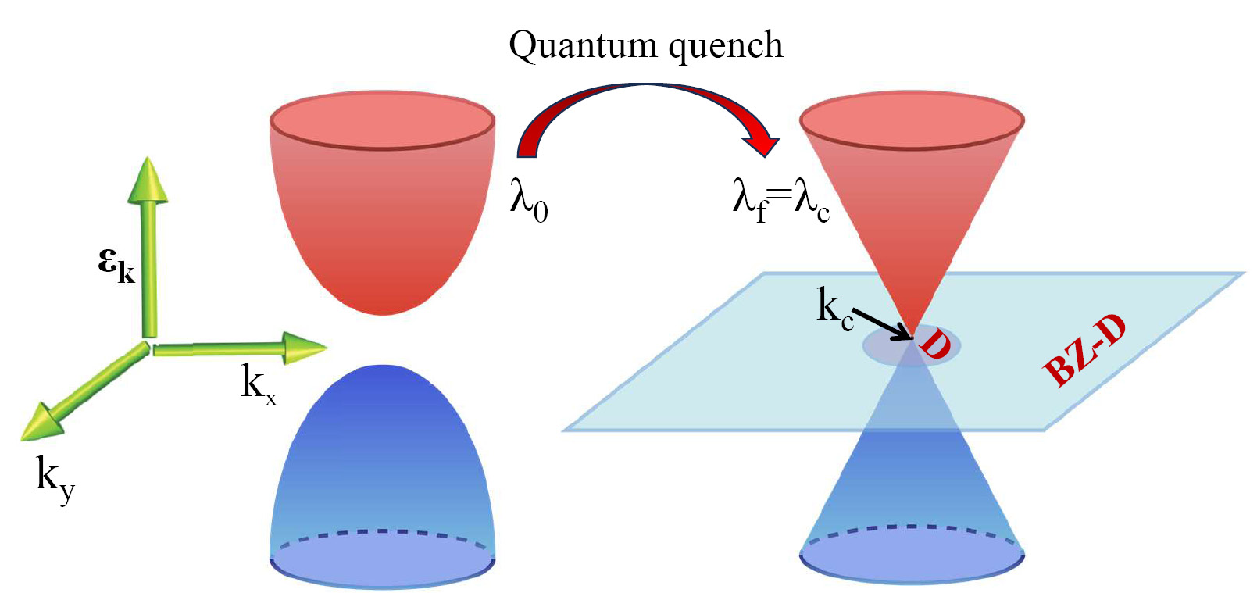
\includegraphics[width=0.7\textwidth]{figures/QV_BZ_D.pdf}
				\bicaption{二维系统量子淬火动力学的示意图。
					阴影部分(区域$D$)表示了第一布里渊区中能隙闭合点$\mathbf{k}_c$附近的邻域。}{Illustration of the quantum quench dynamics in a 2D case.
					The shadowed regime  (denoted by $D$) indicates a small vicinity around the gap close point $\mathbf{k}_c$ in the 1st BZ.} \label{Fig:BZ_D}
			\end{figure} 		
		
			{\bf 第一步:}
			哈密顿矢量${\vec{h}}_{\mathbf{k}}$的解析性允许我们将积分区间从整个第一布里渊区缩小到孤立能隙闭合点的邻域内。
			简单起见,考虑第一布里渊区内只有一个能隙闭合点,我们需要证明:
			\begin{equation}
				\frac{d}{d\lambda_f} \int_{BZ-D} r_\mathbf{k}(\lambda_f) d\mathbf{k} \bigg|_{\lambda_f=\lambda_c^-} - \frac{d}{d\lambda_f} \int_{BZ-D} r_\mathbf{k}(\lambda_f) d\mathbf{k} \bigg|_{\lambda_f=\lambda_c^+}
			\end{equation}
			这一表达式为零。
			其中$D$是$\mathbf{k}_c$附近任意小的邻域。
			对于$D$关于第一布里渊区的补集$BZ-D$,$r_\mathbf{k}^2$是关于$\mathbf{k} \in BZ-D$和$\lambda \in (\lambda_c-\delta \lambda, \lambda_c+\delta \lambda)$双重解析的函数,所以对于$k$的积分和对于$\lambda_f$的导数可以交换:
			\begin{equation}
				\int_{BZ-D} \left(\frac{\partial r_\mathbf{k}(\lambda_f)}{\partial\lambda_f}  \bigg|_{\lambda_f = \lambda_c^-} - \frac{\partial r_\mathbf{k}(\lambda_f)}{\partial\lambda_f} \bigg|_{\lambda_f=\lambda_c^+}\right) d\mathbf{k}. 
			\end{equation}
			
		\subsection{数值结果}
		
				

	\section{结论与展望}